\chapter{Unidad 2. Estructuras del sistema operativo}

\section{Introducción}
El diseño de un sistema operativo depende en gran medida de su finalidad y del tipo de procesos que se desean realizar. Además, es crucial tener en cuenta las necesidades o requisitos del usuario y del propio software.
 A continuación, se detallan estos aspectos fundamentales:

\subsection{Finalidad del Sistema Operativo}

La finalidad de un sistema operativo puede variar según el contexto y los objetivos específicos para los cuales se diseñe. Algunas finalidades comunes incluyen:

\begin{itemize}
	\item \textbf{Gestión de Recursos}: Coordinar y optimizar el uso de los recursos de hardware (CPU, memoria, dispositivos de E/S) para mejorar el rendimiento y la eficiencia del sistema.
	\item \textbf{Interfaz de Usuario}: Proveer una interfaz amigable para que los usuarios interactúen fácilmente con el hardware y el software de la computadora.
	\item \textbf{Seguridad y Protección}: Asegurar que los datos y recursos del sistema estén protegidos contra accesos no autorizados y errores.
	\item \textbf{Compatibilidad y Soporte de Aplicaciones}: Facilitar la ejecución de aplicaciones y programas, proporcionando una plataforma estable y compatible.
\end{itemize}

\subsection{ Tipo de Procesos}

El tipo de procesos que se desea realizar influye significativamente en el diseño del sistema operativo. Algunos ejemplos incluyen:

\begin{itemize}
	\item \textbf{Procesamiento por Lotes}: Adecuado para tareas que pueden agruparse y ejecutarse sin intervención del usuario. Ejemplos: procesamiento de datos en bancos y grandes corporaciones.
	\item \textbf{Tiempo Compartido}: Permite que múltiples usuarios utilicen el sistema simultáneamente, cada uno con la ilusión de tener acceso exclusivo. Ejemplos: sistemas multiusuario en universidades y centros de investigación.
	\item \textbf{Tiempo Real}: Requiere que las operaciones se realicen dentro de un tiempo específico y predecible. Ejemplos: sistemas de control industrial, aviación, y dispositivos médicos.
	\item \textbf{Procesamiento Distribuido}: Involucra la coordinación de múltiples sistemas para trabajar en conjunto. Ejemplos: computación en la nube, sistemas de archivos distribuidos.
\end{itemize}

\subsection{Necesidades del Usuario}

Las necesidades del usuario pueden variar dependiendo del contexto de uso del sistema operativo. Algunas necesidades comunes incluyen:

\begin{itemize}
	\item \textbf{Facilidad de Uso}: Interfaces gráficas intuitivas y fáciles de navegar.
	\item \textbf{Personalización}: Opciones para personalizar el entorno de trabajo según las preferencias del usuario.
	\item \textbf{Soporte Técnico y Documentación}: Acceso a soporte técnico y documentación detallada para resolver problemas y aprender a usar el sistema.
	\item \textbf{Compatibilidad de Software}: Capacidad para ejecutar una amplia variedad de aplicaciones y software específico del usuario.
\end{itemize}

\subsection{ Necesidades del Software}

El software que se ejecutará en el sistema operativo también impone requisitos específicos que deben ser considerados en el diseño. Algunos de estos requisitos incluyen:

\begin{itemize}
	\item \textbf{Gestión de Memoria}: Necesidad de un manejo eficiente de la memoria para ejecutar aplicaciones grandes y complejas.
	\item \textbf{Procesamiento Multitarea}: Capacidad para ejecutar múltiples tareas simultáneamente sin degradación del rendimiento.
	\item \textbf{Control de Dispositivos}: Soporte para una variedad de dispositivos de entrada/salida, como impresoras, escáneres, y dispositivos de almacenamiento externo.
	\item \textbf{Seguridad y Protección de Datos}: Implementación de medidas de seguridad para proteger los datos y asegurar la integridad del sistema.
\end{itemize}



\subsection*{Modos Usuario y Kernel del Sistema Operativo}

\textbf{Modo Usuario}

\begin{itemize}
	\item \textbf{Descripción}: 
	\begin{itemize}
		\item El modo usuario es el modo de operación en el que se ejecutan las aplicaciones y programas del usuario.
		\item Las aplicaciones en este modo tienen acceso limitado a los recursos del sistema y no pueden realizar operaciones críticas de hardware directamente.
		\item El sistema operativo proporciona una capa de protección para evitar que las aplicaciones en modo usuario dañen el sistema o interfieran con otras aplicaciones.
	\end{itemize}

\end{itemize}

\textbf{Modo Kernel}

\begin{itemize}
	\item \textbf{Descripción}:
	\begin{itemize}
		\item El modo kernel es el modo de operación en el que se ejecuta el núcleo del sistema operativo.
		\item Tiene acceso completo a todos los recursos del hardware, incluyendo la memoria, el procesador y los dispositivos de entrada/salida.
		\item Las operaciones críticas del sistema, como la gestión de procesos, la gestión de memoria y el control de dispositivos, se realizan en este modo.
	\end{itemize}

\end{itemize}

\textbf{Comparación}

\begin{itemize}
	\item \textbf{Seguridad}:
	\begin{itemize}
		\item \textbf{Modo Usuario}: Mayor seguridad debido a las restricciones de acceso.
		\item \textbf{Modo Kernel}: Menor seguridad ya que tiene acceso total a los recursos.
	\end{itemize}
	\item \textbf{Acceso a Recursos}:
	\begin{itemize}
		\item \textbf{Modo Usuario}: Acceso limitado; requiere llamadas al sistema para servicios.
		\item \textbf{Modo Kernel}: Acceso completo y directo a todos los recursos del sistema.
	\end{itemize}
	\item \textbf{Propósito}:
	\begin{itemize}
		\item \textbf{Modo Usuario}: Ejecutar aplicaciones y programas del usuario.
		\item \textbf{Modo Kernel}: Gestionar y controlar el hardware y los recursos del sistema.
	\end{itemize}
\end{itemize}


 

\section{Estructura monolítica}

Es la estructura de los primeros sistemas operativos, constituidos fundamentalmente por un solo programa compuesto de un conjunto de rutinas entrelazadas de tal forma que cada una puede llamar a cualquier otra.

\begin{figure}[H]
	\centering
	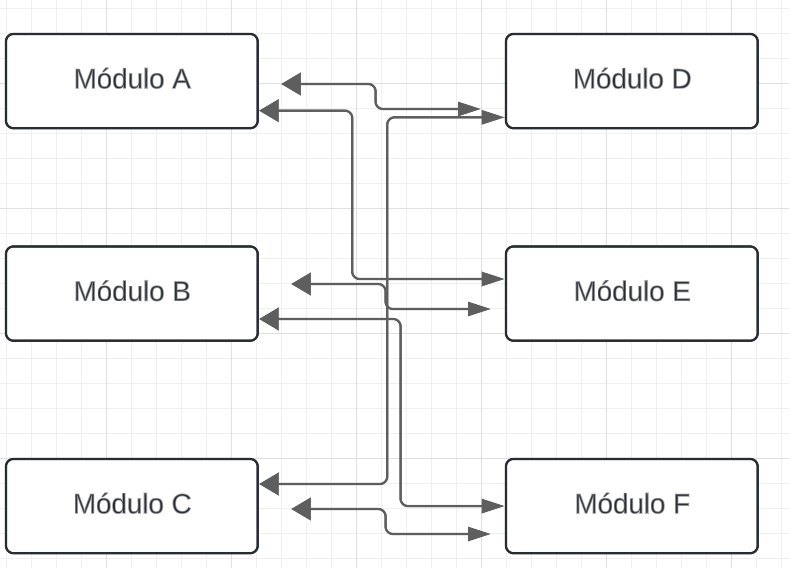
\includegraphics[width=0.6\linewidth]{Imagenes/monolitico.png}
	\caption{En un sistema operativo monolítico sus módulos están entrelazados. }
	\label{fig:enter-label}
\end{figure}

\subsection{Características Fundamentales del Sistema Monolítico}
\begin{tcolorbox}

\subsubsection{Estructura Unificada}
\begin{itemize}
	\item \textbf{Descripción}: El sistema operativo monolítico se compone de un único bloque de código en el que todos los servicios del sistema (gestión de archivos, gestión de memoria, manejo de dispositivos, etc.) están interrelacionados.
	\item \textbf{Funcionalidad}: Todas las funciones del sistema operativo están disponibles en el mismo espacio de direcciones y pueden llamarse entre sí directamente.
\end{itemize}
	
\end{tcolorbox}


\begin{tcolorbox}


\subsubsection{Rendimiento Alto}
\begin{itemize}
	\item \textbf{Descripción}: Al tener todos los servicios en un único espacio de direcciones, las llamadas de función son rápidas.
	\item \textbf{Ventaja}: No hay necesidad de cambiar entre el modo usuario y el modo kernel para acceder a los servicios del sistema operativo, lo que reduce la sobrecarga y mejora el rendimiento.
\end{itemize}
\end{tcolorbox}

\begin{tcolorbox}

\subsubsection{Simplicidad de Implementación}
\begin{itemize}
	\item \textbf{Descripción}: La estructura monolítica es más sencilla de implementar y gestionar, ya que todo el código está contenido en un solo lugar.
	\item \textbf{Beneficio}: Esto facilita la integración de componentes y la comunicación interna, haciendo que el desarrollo inicial del sistema operativo sea más directo.
\end{itemize}

\end{tcolorbox}


\begin{tcolorbox}
	
\subsubsection{Dificultad en la Escalabilidad}
\begin{itemize}
	\item \textbf{Descripción}: Agregar nuevas funciones o servicios puede ser complicado debido a la interdependencia entre los componentes existentes.
	\item \textbf{Reto}: A medida que el sistema operativo crece, mantener y extender el código puede volverse más complejo.
\end{itemize}

\end{tcolorbox}

\begin{tcolorbox}
\subsubsection{Seguridad Reducida}
\begin{itemize}
	\item \textbf{Descripción}: La falta de separación entre los distintos componentes del sistema operativo implica que un fallo en un módulo puede comprometer todo el sistema.
	\item \textbf{Consecuencia}: Esto reduce la robustez y la seguridad del sistema operativo, ya que cualquier error puede afectar a todo el sistema.
\end{itemize}
\end{tcolorbox}


\section{Estructura Jerárquica}



La estructura jerárquica llega como una evolución natural de los sistemas operativos. A medida que crecieron las necesidades de los usuarios y aumentó la complejidad de las aplicaciones, se hizo necesaria una mejor organización del software. 

La estructura jerárquica organiza el sistema operativo en pequeñas partes o capas, cada una de las cuales tiene una función específica y depende de las capas inferiores para realizar sus tareas.
Uno de los ejemplos más conocidos de estructura jerárquica es el modelo THE (Technische Hogeschool, Eindhoven  ) desarrollado por Edsger Dijkstra, y se presenta de la siguiente manera:
\begin{figure}[H]
	\centering
	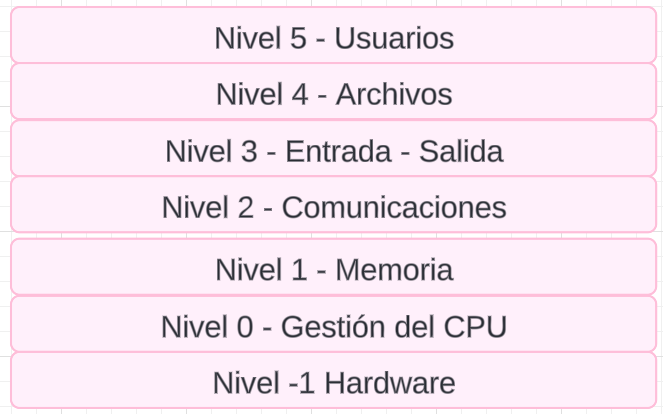
\includegraphics[width=0.6\linewidth]{Imagenes/jerarquico.png}
	\caption{En un sistema operativo monolítico sus módulos están entrelazados. }
	\label{fig:enter-label}
\end{figure}



En la estructura jerárquica, el sistema operativo se divide en capas, donde cada capa proporciona servicios a la capa superior y utiliza los servicios de la capa inferior. La capa más baja interactúa directamente con el hardware, y la capa más alta proporciona la interfaz de usuario.

\begin{tcolorbox}[title=Capas de la estructura jerárquica]


\begin{itemize}
	\item \textbf{Capa -1 (Hardware)}
	\begin{itemize}
		\item \textbf{Función}: Interactúa directamente con el hardware físico del sistema, incluyendo la CPU, la memoria y los dispositivos de E/S.
	\end{itemize}
	
	\item \textbf{Capa 0 (Planificación del Procesador)}
	\begin{itemize}
		\item \textbf{Función}: Controla la ejecución de procesos y la planificación de tareas. Gestiona la creación, terminación y sincronización de procesos.
	\end{itemize}
	
	\item \textbf{Capa 1 (Gestión de la Memoria)}
	\begin{itemize}
		\item \textbf{Función}: Maneja la asignación y el control de la memoria. Proporciona servicios como la asignación de memoria y el intercambio de memoria.
	\end{itemize}
	
	\item \textbf{Capa 2 (Controlador de la Consola de Operador)}
	\begin{itemize}
		\item \textbf{Función}: Gestiona la interacción con la consola del operador, permitiendo la entrada y salida de comandos y datos.
	\end{itemize}
	
	\item \textbf{Capa 3 (Control de Entrada/Salida)}
	\begin{itemize}
		\item \textbf{Función}: Controla los dispositivos de hardware a través de controladores. Gestiona las operaciones de entrada/salida y la comunicación con los periféricos.
	\end{itemize}
	
	\item \textbf{Capa 4 (Gestión de Archivos)}
	\begin{itemize}
		\item \textbf{Función}: Proporciona servicios de sistema de archivos, como la creación, eliminación y manipulación de archivos. Controla el acceso a los datos almacenados en disco.
	\end{itemize}
	
	\item \textbf{Capa 5 (Control de Programas de Usuarios)}
	\begin{itemize}
		\item \textbf{Función}: Gestiona la ejecución y control de los programas de los usuarios, proporcionando una interfaz para la interacción con el sistema operativo.
	\end{itemize}
\end{itemize}
\end{tcolorbox}
\subsection{Características Fundamentales}


\begin{itemize}
	\item \textbf{Modularidad}
	\begin{itemize}
		\item \textbf{Descripción}: Cada capa del sistema operativo está diseñada para cumplir con una función específica, permitiendo que los desarrolladores trabajen en una capa sin afectar las demás.
		\item \textbf{Ventaja}: Facilita el desarrollo, la prueba y el mantenimiento del sistema operativo.
	\end{itemize}
	
	\item \textbf{Independencia de Capas}
	\begin{itemize}
		\item \textbf{Descripción}: Las capas superiores dependen de los servicios proporcionados por las capas inferiores, pero no necesitan conocer los detalles internos de esas capas.
		\item \textbf{Ventaja}: Mejora la confiabilidad y la seguridad del sistema, ya que los cambios en una capa no afectan a las demás.
	\end{itemize}
	
	\item \textbf{Facilidad de Mantenimiento}
	\begin{itemize}
		\item \textbf{Descripción}: La modularidad y la independencia de capas hacen que el sistema operativo sea más fácil de mantener y actualizar.
		\item \textbf{Ventaja}: Las actualizaciones y correcciones de errores pueden realizarse en una capa sin afectar el resto del sistema.
	\end{itemize}
\end{itemize}

\section{Máquina Virtual}
La máquina virtual es una evolución natural de los sistemas operativos que aprovecha la potencia del hardware moderno para aplicar la técnica de multiprogramación y el concepto de máquina extendida. 

Una máquina extendida es una versión virtualizada de una computadora física que presenta una visión más completa y rica de los recursos de hardware. En lugar de interactuar directamente con el hardware físico, los programas y sistemas operativos interactúan con una representación virtual de la máquina.

\begin{figure}[H]
	\centering
	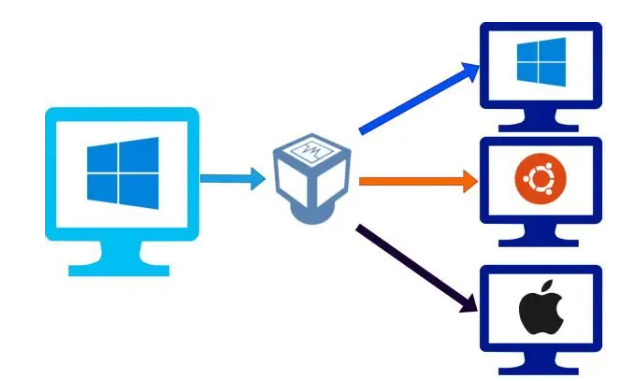
\includegraphics[width=0.6\linewidth]{Imagenes/virtual.png}
	\caption{Una máquina virtual puede ejecutar diferentes s.o. en una computadora. }
	\label{fig:enter-label}
\end{figure}


 Esto permite la integración de distintos sistemas operativos en una sola computadora física, dando la sensación de tener varias máquinas diferentes y permitiendo la ejecución simultánea de múltiples sistemas operativos y aplicaciones.
 
\subsection{Características Fundamentales
}


\begin{itemize}
	\item \textbf{Aislamiento}
	\begin{itemize}
		\item \textbf{Descripción}: Cada máquina virtual es como una burbuja separada, sin afectar a las otras burbujas.
		\item \textbf{Ventaja}: Si una máquina virtual falla, las otras siguen funcionando sin problemas.
	\end{itemize}
	
	\item \textbf{Flexibilidad}
	\begin{itemize}
		\item \textbf{Descripción}: Puedes ejecutar diferentes sistemas operativos al mismo tiempo en la misma computadora.
		\item \textbf{Ventaja}: Esto es útil para pruebas y desarrollo, ya que no necesitas hardware adicional.
	\end{itemize}
	
	\item \textbf{Eficiencia de Recursos}
	\begin{itemize}
		\item \textbf{Descripción}: El monitor de recursos distribuye los recursos (como CPU y memoria) de manera eficiente entre las máquinas virtuales.
		\item \textbf{Ventaja}: Se aprovecha mejor el hardware de la computadora.
	\end{itemize}
	
\end{itemize}

\section{Estructura Cliente-Servidor}



El modelo cliente-servidor es una arquitectura de sistemas operativos y aplicaciones donde las tareas se reparten entre proveedores de recursos o servicios, llamados servidores, y los consumidores de esos servicios, llamados clientes. Este modelo es ampliamente utilizado en redes y permite una distribución eficiente de tareas y recursos.
\begin{figure}[H]
	\centering
	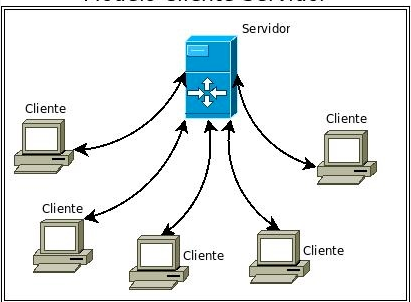
\includegraphics[width=0.7\linewidth]{Imagenes/cliente-servidor.png}
	\caption{El modelo cliente-servidor. }
	\label{fig:enter-label}
\end{figure}


En un sistema operativo cliente-servidor, los servidores son programas que proporcionan servicios específicos, como almacenamiento de datos, procesamiento de aplicaciones, o administración de recursos. Los clientes son programas que solicitan estos servicios. La comunicación entre clientes y servidores se realiza a través de una red.

\subsection{Características Fundamentales}

\begin{itemize}
	\item \textbf{Distribución de Tareas}
	\begin{itemize}
		\item \textbf{Descripción}: Las tareas se reparten entre clientes y servidores. Los servidores gestionan y proporcionan recursos y servicios, mientras que los clientes consumen estos servicios.
		\item \textbf{Ventaja}: Mejora la eficiencia y permite la especialización en la provisión de servicios.
	\end{itemize}
	
	\item \textbf{Independencia de Plataforma}
	\begin{itemize}
		\item \textbf{Descripción}: Los clientes y servidores pueden operar en diferentes plataformas de hardware y sistemas operativos, siempre que se adhieran a protocolos de comunicación comunes.
		\item \textbf{Ventaja}: Facilita la integración de diferentes tecnologías y sistemas.
	\end{itemize}
	
	\item \textbf{Escalabilidad}
	\begin{itemize}
		\item \textbf{Descripción}: Es fácil agregar más servidores o clientes según la demanda, permitiendo una escalabilidad horizontal.
		\item \textbf{Ventaja}: Permite manejar incrementos en la carga de trabajo de manera eficiente.
	\end{itemize}
	
	\item \textbf{Mantenimiento Centralizado}
	\begin{itemize}
		\item \textbf{Descripción}: La gestión y el mantenimiento de los recursos y servicios se centralizan en los servidores.
		\item \textbf{Ventaja}: Facilita la administración y el mantenimiento del sistema.
	\end{itemize}
\end{itemize}

\subsubsection*{Ejemplo de Funcionamiento}

En un sistema cliente-servidor, los clientes envían solicitudes a los servidores a través de la red. Los servidores procesan estas solicitudes y envían las respuestas correspondientes. Por ejemplo:
\begin{itemize}
	\item Un cliente puede solicitar datos de una base de datos al servidor.
	\item El servidor procesa la solicitud, accede a la base de datos, y envía los datos solicitados al cliente.
\end{itemize}

\section{Prestaciones de un sistema operativo}
Se ha mencionado que la misión del sistema operativo es ayudar al usuario con el manejo de la computadora, para eso debe proporcionar ciertos servicios que se pueden considerar desde dos puntos de vista distintos.

\begin{tcolorbox}
\begin{itemize}
	\item Punto de vista del programador
	\item Punto de vista del sistema
\end{itemize}

\end{tcolorbox}

\subsubsection{Punto de vista del programador}
Desde el punto de vista del programador, las prestaciones del sistema operativo son las funcionalidades y servicios que el sistema operativo proporciona para facilitar el desarrollo, ejecución y gestión de programas. 

Estas prestaciones permiten a los programadores enfocarse en la lógica y funcionalidad de sus aplicaciones sin tener que preocuparse por los detalles del hardware y la gestión de recursos subyacentes.

\begin{tcolorbox}
\textbf{Punto de vista del programador}:	funcionalidades del sistema operativo, que facilitan el desarrollo, la ejecución, y gestión de programas.

\subsubsection{Ejecución de programas}
\begin{itemize}
	\item El sistema operativo proporciona servicios que permiten cargar, ejecutar y finalizar programas de manera eficiente.
\end{itemize}

\subsubsection{Operaciones de Entrada/Salida (E/S)}
\begin{itemize}
	\item El sistema operativo maneja las operaciones de entrada y salida, facilitando la interacción entre el software y los dispositivos de hardware.
\end{itemize}

\subsubsection{Gestión de archivos}
\begin{itemize}
	\item El sistema operativo proporciona mecanismos para la creación, acceso y manipulación de archivos en el sistema de archivos.
\end{itemize}

\end{tcolorbox}


\subsubsection{Punto de vista del sistema}
Desde el punto de vista del sistema, las prestaciones del sistema operativo se centran en cómo se gestionan y optimizan los recursos del sistema para garantizar su eficiencia, seguridad y estabilidad. 
\begin{tcolorbox}
	\textbf{Punto de vista del sistema}: Gestión y optimización de recursos.
	
	\subsubsection{Asignación de Recursos}
	\begin{itemize}
		\item La asignación de recursos implica distribuir de manera eficiente la CPU, memoria y otros recursos del sistema entre los programas que se están ejecutando, resolviendo conflictos de asignación cuando varios procesos o usuarios compiten por los mismos recursos.
	\end{itemize}
	
	\subsubsection{Contabilidad}
	\begin{itemize}
		\item La contabilidad en un sistema operativo se refiere al registro y monitoreo del uso de recursos por parte de los diferentes procesos y usuarios.
	\end{itemize}
	
	\subsubsection{Protección}
	\begin{itemize}
		\item La protección en un sistema operativo implica asegurar que los datos y recursos del sistema no sean accesibles de manera indebida o por usuarios no autorizados.
	\end{itemize}
	
\end{tcolorbox}

\subsection{Servicios de usuario}
El sistema operativo ofrece servicios a los usuarios de dos formas diferentes: a través de llamadas al sistema operativo desde un proceso y mediante la ejecución de programas del propio sistema operativo. 

	\subsubsection{Llamadas al sistema operativo desde un proceso}
Las llamadas al sistema operativo son interfaces que permiten a los programas solicitar servicios específicos del sistema operativo. Estas llamadas se agrupan en varias categorías:
\begin{tcolorbox} 
	
		\begin{enumerate}
			\item\textbf{ Gestión de procesos}: Permiten crear, gestionar y terminar procesos. 
			\begin{lstlisting}
				exit()
			\end{lstlisting}
			
			\textit{Cuando cierras una aplicación.}
			 \item \textbf{Gestión de operaciones de E/S}: Permiten realizar operaciones de entrada y salida.
		\begin{lstlisting}
			read()
		\end{lstlisting}
		\textit{Cuando abres un archivo de word.}

		
		\item \textbf{Gestión de sistema de archivos}: Permiten manipular archivos y directorios. 
		\begin{lstlisting}
			mkdir ejemplo
		\end{lstlisting}
		
		\textit{Cuando creas una carpeta.}
		\end{enumerate}

\end{tcolorbox}
	
	
	\subsubsection{Ejecución de programas del propio sistema operativo}
	Además de las funciones básicas del núcleo que pueden ser ejecutadas por medio de llamadas al sistema, el sistema operativo proporciona un conjunto de programas cuya misión es resolver problemas comunes de los usuarios. 
	
	Estos programas se agrupan en varias categorías y facilitan la interacción con el sistema, proporcionando herramientas útiles para la gestión y manipulación de datos.
	
	\begin{tcolorbox}
	\begin{enumerate}
	\item\textbf{Tratamiento de Archivos }:Programas que permiten manipular archivos, tales como copiar, mover, renombrar y eliminar archivos.

	\begin{lstlisting}
		cp ejemplo.txt ejemplo1.txt
	\end{lstlisting}
	 \textit{Copia archivos de un lugar a otro}
	 
	 \item \textbf{Información}: Programas que proporcionan información sobre el sistema y los archivos, ayudando a los usuarios a entender el estado y uso de los recursos del sistema. 

		\begin{lstlisting}
		ls %Lista los archivos en un directorio
		df %Muestra el espacio disponible en disco
	\end{lstlisting}
	

	
	\item \textbf{Editores}:  Programas que permiten editar archivos de texto, proporcionando interfaces desde simples a muy sofisticadas. 

	\begin{lstlisting}
		nano ejemplo.txt
	\end{lstlisting}
	\textit{Cuando creas una carpeta.}
	
	\item \textbf{Ejecución}: Programas que permiten ejecutar y gestionar otros programas.
		\begin{lstlisting}
		python ejemplo.py
		sh script.sh
	\end{lstlisting}
	
		\item \textbf{Interprete de comandos}: Programas que interpretan y ejecutan comandos ingresados por el usuario, proporcionando una interfaz interactiva para el control del sistema.
	\begin{lstlisting}
		$ bash
		$ echo "Hola, mundo!"
		$ ls -la
	\end{lstlisting}
	
		\item \textbf{Programas de utilidad}: Programas que realizan tareas comunes de mantenimiento y gestión del sistema.
	\begin{lstlisting}
		$ grep "hola" ejemplo.txt
		$ Busca la palabra "hola" en el archivo
		
	\end{lstlisting}
\end{enumerate}
	

\end{tcolorbox}

\subsection{Servicios del sistema}

El sistema operativo actúa como un programa activado por eventos, respondiendo a diversas llamadas del sistema y manejando interrupciones y excepciones.
\subsubsection{Llamadas al sistema operativo}
	
Las llamadas al sistema operativo se agrupan según el tipo de llamada y  no por las acciones que realizan. Estas llamadas permiten a los programas interactuar con el núcleo del sistema operativo para realizar operaciones específicas.

	\begin{tcolorbox}
	\begin{enumerate}
		\item\textbf{Terminación normal }:Llamadas que permiten a un proceso finalizar su ejecución de manera controlada.
		
		\begin{lstlisting}
			exit()
		\end{lstlisting}
		\textit{El comando exit() es una llamada que finaliza el proceso actual y libera los recursos asignados.}
		
		\item\textbf{Terminación anormal }: Ocurre cuando un proceso termina debido a un error o una condición inesperada.
		
		\begin{lstlisting}
			Exception in thread "main" java.lang.NullPointerException
			at tu.paquete.TuClase.tuMetodo(TuClase.java:numeroDeLinea)
		\end{lstlisting}
		
		
		
		\textit{Cuando un programa Java intenta utilizar un objeto que no ha sido inicializado (es decir, que apunta a null), se lanza una NullPointerException. }
		
		\item \textbf{Peticiones de estado}: Llamadas que solicitan información sobre el estado del sistema, procesos u otros recursos. Se procesa la petición solicitada y se devuelve el control al programa que la solicitó.
		
		\begin{lstlisting}
			# Obtener el ID del proceso actual
			pid=$$
			# Imprimir el ID del proceso actual
			echo "El ID del proceso actual es: $pid"
		\end{lstlisting}
		
		
		
		\item \textbf{Peticiones de recursos}:  Los programas que son ejecutados, solicitan la asignación o liberación de recursos, y serán atendidos inmediatamente o entrarán en un estado de espera hasta ser atendidos.
	
		
		\item \textbf{Peticiones de E/S}: Llamadas que solicitan operaciones de entrada/salida, como leer o escribir datos.
		\begin{lstlisting}
			nombre = input('ingrese su nombre')
			print(nombre)
		\end{lstlisting}
		
	
	\end{enumerate}
	
	
\end{tcolorbox}

\subsubsection{Interrupciones de los Dispositivos de E/S}
Las interrupciones son señales enviadas por dispositivos de E/S al procesador para indicar que requieren atención. El sistema operativo maneja estas interrupciones y decide la acción a tomar.

Pueden ser:
	\begin{tcolorbox}
	\begin{enumerate}
		\item\textbf{Quedando en espera }:El proceso se suspende y espera a que el dispositivo esté listo para continuar. En este caso, el dispositivo externo, cuando termine la operación, producirá una interrupción que dará control al sistema operativo, el cual activará el proceso que estaba en espera.
		
	
		\textit{ \textbf{Ejemplo:} Un proceso que espera a que un disco duro termine de escribir datos antes de continuar con su ejecución.}
		
		\item\textbf{Siguiendo con las operaciones }:  El proceso principal continúa ejecutándose mientras el sistema operativo maneja las interrupciones en segundo plano. Esto permite que la computadora realice múltiples tareas al mismo tiempo.
		
	
		\textit{\textbf{Ejemplo}: Estás imprimiendo un documento mientras sigues trabajando en otros programas. La impresora envía una interrupción cuando termina de imprimir cada página, pero tu trabajo no se detiene. }
		
	
		
		
	\end{enumerate}
	
	
\end{tcolorbox}

\subsubsection{Gestión de excepciones}
La gestión de excepciones es un mecanismo para manejar condiciones excepcionales, como errores de hardware o software, que ocurren durante la ejecución de un programa.

\textit{El sistema operativo detecta la excepción, interrumpe la ejecución del programa, y ejecuta un manejador de excepciones.
}

\subsection{Protecciones del sistema operativo}
Las protecciones en el sistema operativo son funciones implementadas para evitar problemas entre procesos y entre estos y el propio sistema operativo. Estas protecciones aseguran que los procesos no interfieran entre sí y que el sistema operativo mantenga su integridad y estabilidad. Existen varios tipos de protecciones, entre las cuales se incluyen la protección de entrada/salida (E/S), la protección de memoria y la protección del procesador.


	\begin{enumerate}
			\begin{tcolorbox}
		\item\textbf{Protección de Entrada/Salida (E/S)}: Garantiza que las operaciones de E/S sean seguras y controladas, evitando que los procesos interfieran con los dispositivos de E/S de otros procesos. Solo los procesos autorizados pueden acceder a dispositivos de E/S específicos.
		
		\textit{ \textbf{Ejemplo:}Un sistema operativo que utiliza permisos para controlar el acceso a una impresora, asegurando que solo ciertos usuarios o procesos puedan enviar trabajos de impresión.}
		
		\item\textbf{Protección de Memoria}: Previene que los procesos accedan a áreas de memoria que no les pertenecen, evitando corrupción de datos y fallos del sistema.
		
			
		\item\textbf{Protección del Procesador}: Asegura que ningún proceso pueda monopolizar el procesador, garantizando una distribución justa del tiempo de CPU entre todos los procesos.
		Utiliza temporizadores y modos de operación (modo usuario y modo kernel) para controlar el uso del procesador.
		
		
	\end{tcolorbox}
		
	\end{enumerate}
	
	

 















